\documentclass[10pt]{beamer}

\usepackage{pgfpages}
%\setbeameroption{show notes on second screen}

\usetheme{metropolis}
\usepackage{appendixnumberbeamer}

\usepackage{booktabs}
\usepackage[scale=2]{ccicons}

\usepackage{pgfplots}
\usepgfplotslibrary{dateplot}

\usepackage{xspace}
\newcommand{\themename}{\textbf{\textsc{metropolis}}\xspace}

\usepackage{graphicx}
\usepackage{listings}

\usepackage{lmodern}

\usepackage{eurosym}
\usepackage{amsmath, amssymb}
\usepackage[binary-units=true]{siunitx}
\DeclareSIUnit{\EUR}{\text{\euro}}

\usepackage{xcolor}
\newcommand\crule[3][black]{\textcolor{#1}{\rule{#2}{#3}}}
\definecolor{aswe-reactive}{cmyk}{1,0.9,0,0}
\definecolor{aswe-proactive}{cmyk}{0.6,0.9,0,0}
\definecolor{aswe-preferences}{cmyk}{0,0.75,1,0}
\definecolor{aswe-data}{cmyk}{0.85,0.1,1,0}

\title{ASWE Presentation \#2}
\subtitle{}
\date{\today}
\author{\textbf{Erik Zeiske}, \textbf{Leon Schürmann}, Andreas Fuchs, Anne Born, Dorian Czichotzki and Thore Krüss}
% \titlegraphic{\hfill\includegraphics[height=1.5cm]{logo.pdf}}

\begin{document}

\maketitle

\begin{frame}{Agenda}
%  \begin{enumerate}
%    \item Reworked architecture
%      \begin{itemize}
%        \item API documentation
%        \item Information flow
%      \end{itemize}
%    \item Design patterns
%    \item Demo
%  \end{enumerate}
  \tableofcontents
\end{frame}

\section{Reworked architecture}

\begin{frame}{Old architecture}
  \includegraphics[width=0.85\textwidth]{architecture_old}
\end{frame}

\begin{frame}{Old architecture}
  \begin{itemize}
    \item Design was \textit{push-based}
    \item Reactive behaviour difficult
    \item Data-oriented instead of request-oriented
  \end{itemize}
  Example:
  \begin{itemize}
    \item \textit{`I'd like to travel to the Airport`}
    \item Set preference: Travel requests $\rightarrow$ DHBW to Airport
    \item Poll \& wait for information store
    \item Respond \only<2>{\textit{... after 5 minutes or so}}
  \end{itemize}
\end{frame}

\begin{frame}{Reworked architecture}
  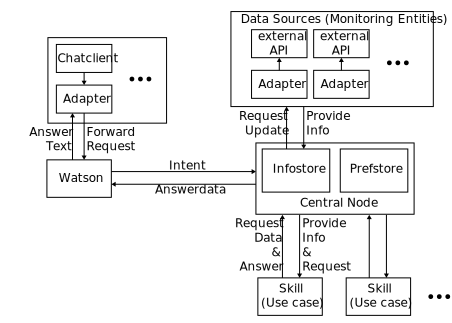
\includegraphics[width=\textwidth]{architecture}
\end{frame}

\subsection{Information flow}

\begin{frame}{Reactive information flow}
  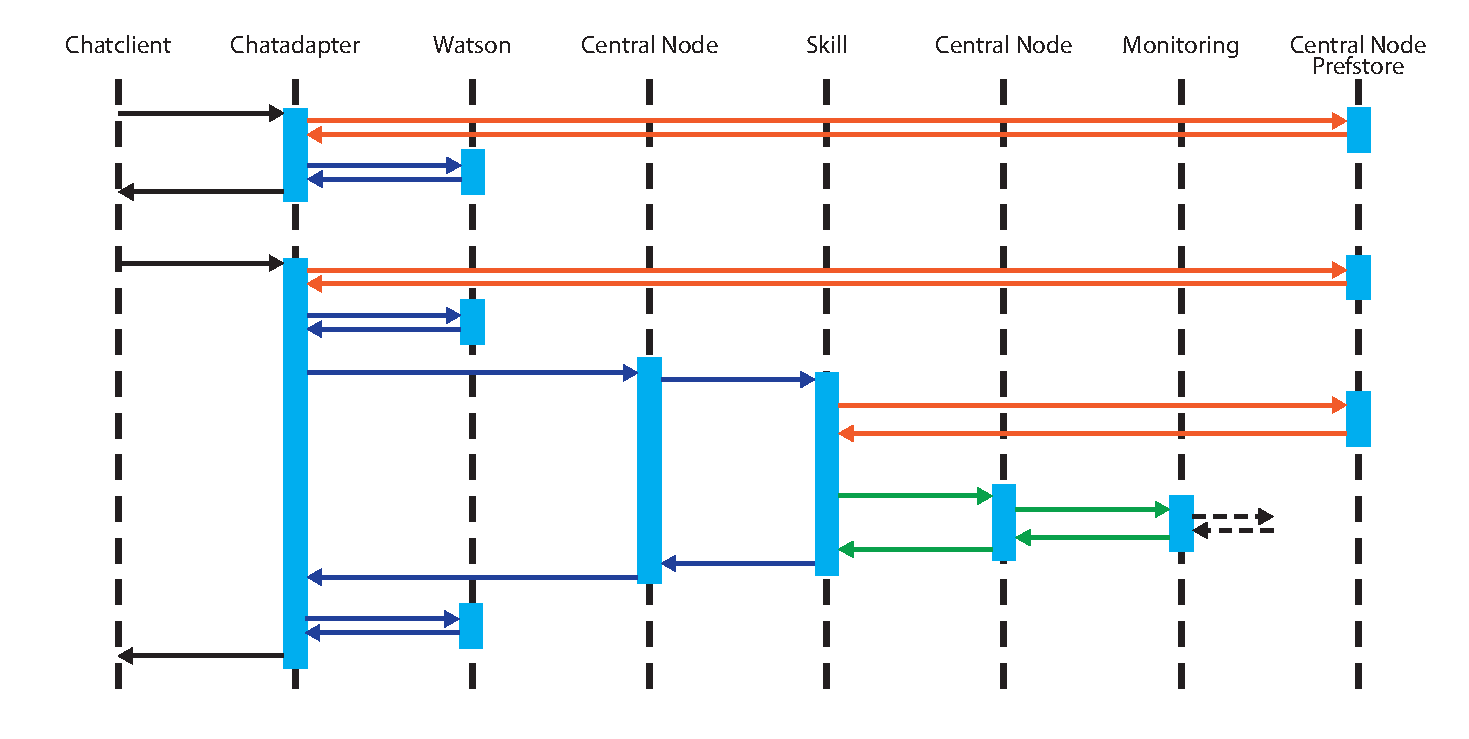
\includegraphics[width=\textwidth,page=1]{ProcessFlows}

  \crule[aswe-reactive]{0.2cm}{0.2cm} Reactive \hspace{0.3cm}
  \crule[aswe-proactive]{0.2cm}{0.2cm} Proactive \hspace{0.3cm}
  \crule[aswe-data]{0.2cm}{0.2cm} Additional Data \hspace{0.3cm}
  \crule[aswe-preferences]{0.2cm}{0.2cm} Preferences
  
\end{frame}

\begin{frame}{Proactive information flow}
  \includegraphics[width=\textwidth,page=2]{ProcessFlows}
  
  \crule[aswe-reactive]{0.2cm}{0.2cm} Reactive \hspace{0.3cm}
  \crule[aswe-proactive]{0.2cm}{0.2cm} Proactive \hspace{0.3cm}
  \crule[aswe-data]{0.2cm}{0.2cm} Additional Data \hspace{0.3cm}
  \crule[aswe-preferences]{0.2cm}{0.2cm} Preferences
\end{frame}

\subsection{API Documentation}

\begin{frame}
  \begin{center}
    \Large \textit{API DOCUMENTATION}
  \end{center}
\end{frame}

\section{Tests}

\begin{frame}[fragile]
  \begin{lstlisting}[language=Python,basicstyle=\footnotesize\ttfamily]
def test_intentInput(self, client, skill):
  body = {
    'skill' : skill,
    'payload' : {},
    'user_handle' : 'AntonHynkel',
    'input_service' : 'Volksempfaenger'
  }
  response = client.post('/api/v1/request', json=body)
  assert response.status_code == 200
  \end{lstlisting}
  \includegraphics[width=\textwidth]{CodeCoverage}
\end{frame}

\section{Design patterns}

\begin{frame}{Design patterns (architectural)}
  \begin{itemize}
    \item Broker pattern
    \item Publish-subscribe
    \item Adapter pattern
  \end{itemize}
\end{frame}

\begin{frame}{Broker pattern}
  \begin{itemize}
    \item Components publish capabilites to a central broker
      \only<2->{
      \begin{itemize}
        \item \textit{Monitoring entities} register to \textit{central node} with \textit{capabilites}
      \end{itemize}
      }
    \item Broker coordinates communication accross components
      \only<3->{
      \begin{itemize}
        \item Bidirectional communication of \textit{skills} and \textit{monitoring entities} through \textit{central node}
      \end{itemize}
      }
    \item Clients access \textit{services}, not servers directly
      \only<4->{
      \begin{itemize}
        \item \textit{Monitoring entities} map their task to abstract \textit{concerns}
      \end{itemize}
      }
  \end{itemize}
\end{frame}

\note[itemize]{
  \item For reactive behaviour
}

\begin{frame}{Publish-subscribe pattern}
  \begin{itemize}
    \item Unidirectional messaging pattern
    \item Senders don't know receivers
      \only<2->{
        \begin{itemize}
          \item \textit{Monitoring entities} don't know which \textit{skills} are interested
        \end{itemize}
      }
    \item Messages belong topic
      \only<3->{
        \begin{itemize}
          \item Represented as a \textit{concern}
          \item Well defined message formats
        \end{itemize}
      }
    \item Receivers actively subscribe to topic
      \only<4->{
        \begin{itemize}
          \item Skills specify \textit{interests} on startup at \textit{central node}
        \end{itemize}
      }
  \end{itemize}
\end{frame}

\note[itemize]{
  \item For proactive behaviour
}

\begin{frame}{Adapter pattern}
  \begin{itemize}
    \item Bridge between two incompatible interfaces
      \only<2->{
        \begin{itemize}
          \item \textit{Chat adapters} accomodate for differences in chat behaviour
        \end{itemize}
      }
    \item Providing a well defined interface
      \only<3->{
        \begin{itemize}
          \item \textit{Monitoring entities} have a well-defined API
        \end{itemize}
      }
  \end{itemize}
\end{frame}
\note[itemize]{
  \item Differences in chat behaviour -> user mentions, replies, etc...
}

%\begin{frame}{Design patterns (code)}
%  \begin{itemize}
%    \item Singleton pattern
%  \end{itemize}
%\end{frame}

%\begin{frame}{Singleton 

\section{Demo}

\begin{frame}
  \begin{center}
    \Large \textit{DEMO}
  \end{center}
\end{frame}
\note[itemize]{
  \item Start with initialization routine
  \item \textit{Multi user support}
}

  
\end{document}
